\documentclass[11pt,aspectratio=169]{beamer}

\usepackage{booktabs}
\usepackage{array}
\usepackage{tikz}
\usepackage{pgfplots}
\usepackage{xcolor}
\usepackage{amsmath}
\usepackage{mathtools}
\usepackage{listings}
\usetikzlibrary{positioning,calc,arrows.meta,decorations.pathreplacing}
\pgfplotsset{compat=1.18}

\usetheme[titleformat=smallcaps,progressbar=frametitle]{metropolis}
\definecolor{UTburnt}{HTML}{BF5700}
\definecolor{LBJnavy}{HTML}{172A46}
\definecolor{softgray}{HTML}{F2F3F5}
\definecolor{midgray}{HTML}{6B7280}
\definecolor{softorange}{HTML}{F9E7DA}
\setbeamercolor{alerted text}{fg=UTburnt}
\setbeamercolor{frametitle}{bg=LBJnavy,fg=white}
\setbeamercolor{progress bar}{fg=UTburnt,bg=gray!25}
\setbeamercolor{block title}{bg=LBJnavy!10,fg=LBJnavy}
\setbeamercolor{block body}{bg=softgray}
\setbeamertemplate{navigation symbols}{}
\setbeamertemplate{itemize item}{\color{UTburnt}$\blacktriangleright$}
\setbeamertemplate{itemize subitem}{\color{UTburnt}$\bullet$}

\lstset{
  basicstyle=\ttfamily\scriptsize,
  backgroundcolor=\color{softgray},
  frame=single,
  rulecolor=\color{midgray!40},
  columns=fullflexible,
  keepspaces=true,
  showstringspaces=false
}

\author{Sergio I. Garc\'ia-R\'ios}
\title{Confidence Intervals}
\subtitle{From sampling uncertainty to a range of plausible values}
\institute{PA 311N: Data Analysis for Public Policy\\LBJ School of Public Affairs}
\date{October 12, 2026}

\newcommand{\yourturn}[1]{%
\begin{center}
\begin{minipage}{0.90\textwidth}
\begin{alertblock}{Your Turn}
#1
\end{alertblock}
\end{minipage}
\end{center}}

\newcommand{\ourturn}[1]{%
\begin{center}
\begin{minipage}{0.90\textwidth}
\begin{block}{Our Turn}
#1
\end{block}
\end{minipage}
\end{center}}

\newcommand{\SE}{\operatorname{SE}}

\begin{document}

% 1
\begin{frame}[plain]
\centering
\vspace{0.6cm}
{\color{LBJnavy}\LARGE\bfseries Confidence Intervals\par}
\vspace{0.4cm}
{\large From sampling uncertainty to a range of plausible values\par}
\vspace{0.9cm}
{\normalsize Sergio I. Garc\'ia-R\'ios\par}
\vspace{0.2cm}
{\small PA 311N: Data Analysis for Public Policy\par}
{\small LBJ School of Public Affairs\par}
\vfill
{\small October 12, 2026\par}
\end{frame}

% 2
\begin{frame}{Where we left off}
Last time we learned that a sample statistic varies from sample to sample.

\[
\bar{x}\ \text{changes, but its sampling distribution is predictable.}
\]

For a sample mean,
\[
\SE(\bar{x}) \approx \frac{s}{\sqrt{n}}.
\]

\vspace{0.8em}
Today we use that sampling uncertainty to move from a \alert{single estimate} to a \alert{range of plausible values} for the population parameter.
\end{frame}

% 3
\begin{frame}{A point estimate hides uncertainty}
Suppose a random sample of 50 Ames homes gives
\[
\bar{x}=1520\text{ sq. ft.}
\]

Is the population mean exactly 1520 square feet?

\vspace{0.8em}
No. Another random sample would probably give a different $\bar{x}$.

\vfill
\begin{alertblock}{The inferential question}
How far from the sample estimate might the true population mean reasonably be?
\end{alertblock}
\end{frame}

% 4
\begin{frame}[standout]
\Large Estimate $\pm$ uncertainty
\end{frame}

% 5
\begin{frame}{The general confidence-interval architecture}
A confidence interval has two pieces:

\[
\boxed{\text{point estimate} \ \pm\ \text{margin of error}}
\]

and

\[
\boxed{\text{margin of error}=\text{critical value}\times\text{standard error}}
\]

So the generic form is
\[
\boxed{\text{estimate}\pm(\text{critical value})(\SE)}
\]

\vfill
\alert{The estimate tells us where to center the interval. The margin of error tells us how far to extend it.}
\end{frame}

% 6
\begin{frame}{Why about two standard errors?}
If the sampling distribution is approximately normal,

\begin{center}
\begin{tikzpicture}
\begin{axis}[
  width=0.82\textwidth,height=0.43\textheight,
  xmin=-3.5,xmax=3.5,ymin=0,ymax=.43,
  axis lines=middle,ytick=\empty,xtick={-2,0,2},
  xticklabels={$\mu-2SE$,$\mu$,$\mu+2SE$},
  tick label style={font=\small}
]
\addplot[LBJnavy,very thick,domain=-3.5:3.5,samples=160] {1/sqrt(2*pi)*exp(-x^2/2)};
\addplot[draw=none,fill=UTburnt!22,domain=-1.96:1.96,samples=120] {1/sqrt(2*pi)*exp(-x^2/2)} \closedcycle;
\draw[<->,UTburnt,very thick] (axis cs:-1.96,.09)--(axis cs:1.96,.09);
\node[UTburnt,font=\large] at (axis cs:0,.14) {about 95\%};
\end{axis}
\end{tikzpicture}
\end{center}

About 95\% of sample means fall within roughly 2 standard errors of $\mu$.

\vfill
Turn that logic around: an interval extending roughly 2 SEs around $\bar{x}$ will capture $\mu$ about 95\% of the time.
\end{frame}

% 7
\begin{frame}{What 95\% confidence means}
Imagine repeating the entire study many times:

\begin{enumerate}
  \item draw a random sample;
  \item calculate a sample mean;
  \item build a 95\% confidence interval using the same procedure.
\end{enumerate}

\vspace{0.8em}
\begin{center}
\Large About \alert{95\% of those intervals} would contain the true population mean.
\end{center}

\vfill
\begin{block}{Confidence is about the procedure}
The population parameter is fixed. The interval changes from sample to sample.
\end{block}
\end{frame}

% 8
\begin{frame}{Repeated intervals: most capture $\mu$, some miss}
\centering
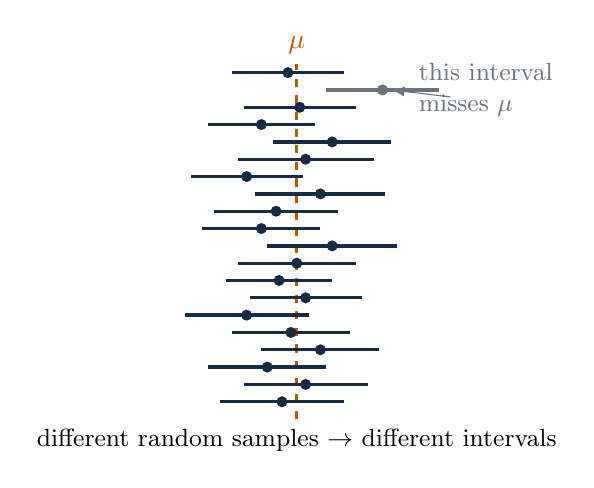
\begin{tikzpicture}[x=0.075cm,y=0.22cm]
\draw[very thick,UTburnt,dashed] (50,0)--(50,20.5);
\node[UTburnt,above] at (50,20.5) {$\mu$};
\foreach \y/\lo/\hi in {
1/37/58,2/41/62,3/35/55,4/44/64,5/39/59,
6/31/52,7/42/61,8/38/56,9/40/60,10/45/67,
11/34/54,12/36/57,13/43/65,14/32/51,15/40/63,
16/46/66,17/35/53,18/41/60,19/55/74,20/39/58}{
  \ifnum\y=19
    \draw[very thick,midgray] (\lo,\y)--(\hi,\y);
    \fill[midgray] ({(\lo+\hi)/2},\y) circle (2pt);
  \else
    \draw[very thick,LBJnavy] (\lo,\y)--(\hi,\y);
    \fill[LBJnavy] ({(\lo+\hi)/2},\y) circle (2pt);
  \fi
}
\node[align=left,font=\small,midgray] at (82,19) {this interval\\misses $\mu$};
\draw[-{Latex},midgray] (76,18.6)--(66,19);
\node[below,font=\small] at (50,0) {different random samples $\rightarrow$ different intervals};
\end{tikzpicture}

\vspace{0.4em}
A 95\% method is allowed to miss sometimes.
\end{frame}

% 9
\begin{frame}{A common misinterpretation}
\begin{alertblock}{Incorrect}
``There is a 95\% probability that $\mu$ lies inside this particular interval.''
\end{alertblock}

\vspace{0.7em}
In the frequentist framework, after we calculate the interval:
\begin{itemize}
  \item $\mu$ is fixed;
  \item the interval either contains $\mu$ or it does not.
\end{itemize}

\vspace{0.7em}
A useful interpretation is:

\begin{center}
\large We are \alert{95\% confident} because this procedure captures the true parameter in about 95\% of repeated random samples.
\end{center}
\end{frame}

% 10
\begin{frame}{Confidence interval for a population mean}
If the population standard deviation $\sigma$ were known,
\[
\bar{x}\pm z^*\frac{\sigma}{\sqrt{n}}.
\]

But in real applications, $\sigma$ is almost never known.

\vspace{0.8em}
We estimate it with the sample standard deviation $s$:
\[
\SE(\bar{x})\approx\frac{s}{\sqrt{n}}.
\]

That extra estimation uncertainty changes the critical value we use.
\end{frame}

% 11
\begin{frame}{When $\sigma$ is unknown: use the $t$ distribution}
For a confidence interval for a population mean,

\[
\boxed{\bar{x}\pm t^*_{df}\frac{s}{\sqrt{n}}}
\]

where
\[
\boxed{df=n-1}.
\]

\vspace{0.7em}
The $t$ distribution is like the normal distribution, but with heavier tails.

\vfill
\alert{For large samples, $t$ and $z$ become very similar.}
\end{frame}

% 12
\begin{frame}{$t$ vs. normal}
\begin{center}
\begin{tikzpicture}
\begin{axis}[
  width=0.82\textwidth,height=0.52\textheight,
  xmin=-4,xmax=4,ymin=0,ymax=.43,
  axis lines=left,ytick=\empty,xtick={-3,-2,-1,0,1,2,3},
  legend style={at={(0.98,0.97)},anchor=north east,font=\small,draw=none}
]
\addplot[LBJnavy,very thick,domain=-4:4,samples=180] {1/sqrt(2*pi)*exp(-x^2/2)};
\addlegendentry{Normal}
\addplot[UTburnt,very thick,dashed,domain=-4:4,samples=180] {0.375*(1+x^2/5)^(-3)};
\addlegendentry{$t$, small df}
\end{axis}
\end{tikzpicture}
\end{center}

The heavier tails make $t^*$ slightly larger than $z^*$ when $n$ is small.
\end{frame}

% 13
\begin{frame}{Critical values depend on confidence level}
For a normal distribution:

\begin{center}
\renewcommand{\arraystretch}{1.25}
\begin{tabular}{ccc}
\toprule
\textbf{Confidence level} & \textbf{Central area} & $\mathbf{z^*}$ \\
\midrule
90\% & 0.90 & 1.645 \\
95\% & 0.95 & 1.960 \\
99\% & 0.99 & 2.576 \\
\bottomrule
\end{tabular}
\end{center}

\vspace{0.8em}
For a mean with unknown $\sigma$, use the corresponding $t^*$ for $df=n-1$.

\vfill
\alert{More confidence requires a larger critical value.}
\end{frame}

% 14
\begin{frame}{Conditions still matter}
Confidence intervals based on the CLT inherit the same conditions we discussed last week.

\begin{enumerate}
  \item \textbf{Independence / random sampling}
  \begin{itemize}
    \item random sampling helps;
    \item if sampling without replacement, $n$ should be less than about 10\% of the population.
  \end{itemize}
  \item \textbf{Nearly normal sampling distribution}
  \begin{itemize}
    \item population roughly normal, or
    \item sample large enough that the CLT works well;
    \item more skewness/outliers require a larger $n$.
  \end{itemize}
\end{enumerate}

\vfill
\alert{A formula cannot repair a badly designed sample.}
\end{frame}

% 15
\begin{frame}[standout]
\Large Let's build one from start to finish.
\end{frame}

% 16
\begin{frame}{Ames example: one sample of 50 homes}
Suppose an illustrative random sample gives

\[
\bar{x}=1520\text{ sq. ft.},\qquad s=500\text{ sq. ft.},\qquad n=50.
\]

We want a 95\% confidence interval for the population mean living area $\mu$.

\vspace{0.8em}
Because $\sigma$ is unknown:
\[
df=50-1=49.
\]

\vfill
The interval is
\[
\bar{x}\pm t^*_{49}\frac{s}{\sqrt{50}}.
\]
\end{frame}

% 17
\begin{frame}{Step 1: calculate the standard error}
\[
\SE(\bar{x})=\frac{s}{\sqrt{n}}
=\frac{500}{\sqrt{50}}
\approx \boxed{70.71\text{ sq. ft.}}
\]

\vspace{0.9em}
Interpretation:

\begin{center}
Across repeated random samples of 50 homes, sample means typically vary by about \alert{71 square feet} around the population mean.
\end{center}
\end{frame}

% 18
\begin{frame}{Step 2: find the critical value}
For a 95\% confidence interval with $df=49$,

\[
t^*_{49}\approx\boxed{2.01}.
\]

In R:
\[\texttt{qt(0.975, df = 49)}\]

Why 0.975?
\[
95\%\text{ in the middle }\Rightarrow 2.5\%\text{ in each tail.}
\]
\end{frame}

% 19
\begin{frame}{Step 3: calculate the margin of error}
\[
ME=t^*\times\SE
\]

\[
ME=2.01(70.71)\approx\boxed{142.1\text{ sq. ft.}}
\]

\vspace{0.8em}
The margin of error is the distance from the point estimate to either endpoint.

\vfill
\begin{center}
\large $1520\ \pm\ 142.1$
\end{center}
\end{frame}

% 20
\begin{frame}{Step 4: construct the interval}
\[
1520\pm142.1
\]

\[
\boxed{(1377.9,\ 1662.1)}
\]

\vspace{0.8em}
\begin{alertblock}{Interpretation}
Using this method, we are 95\% confident that the population mean above-ground living area of Ames homes lies between about 1,378 and 1,662 square feet.
\end{alertblock}

\vfill
For this teaching dataset, the known population mean is 1499.69 square feet, which falls inside the interval.
\end{frame}

% 21
\begin{frame}{Your turn: identify every piece}
\yourturn{A sample of $n=64$ permit applications has mean processing time $\bar{x}=31.2$ days and standard deviation $s=8.0$ days.

For a 95\% confidence interval:
\begin{enumerate}
  \item What is the standard error?
  \item What are the degrees of freedom?
  \item What role does $t^*$ play?
  \item What would the margin of error represent in context?
\end{enumerate}}
\end{frame}

% 22
\begin{frame}{Confidence level and interval width}
Holding the sample and standard error fixed:

\begin{center}
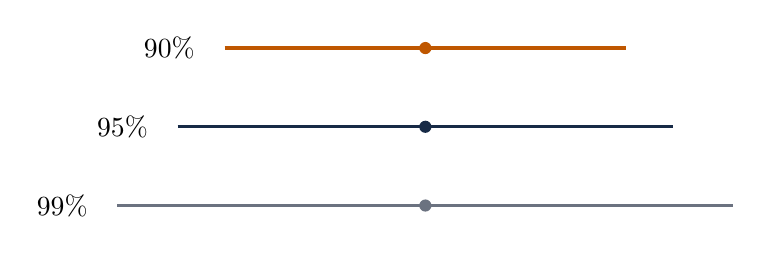
\begin{tikzpicture}[x=0.85cm,y=1cm]
\draw[very thick,UTburnt] (2,2.2)--(8,2.2);
\fill[UTburnt] (5,2.2) circle (2.2pt);
\node[left] at (1.7,2.2) {90\%};
\draw[very thick,LBJnavy] (1.3,1.2)--(8.7,1.2);
\fill[LBJnavy] (5,1.2) circle (2.2pt);
\node[left] at (1.0,1.2) {95\%};
\draw[very thick,midgray] (0.4,0.2)--(9.6,0.2);
\fill[midgray] (5,0.2) circle (2.2pt);
\node[left] at (0.1,0.2) {99\%};
\end{tikzpicture}
\end{center}

\vspace{0.7em}
\[
\text{higher confidence}\Rightarrow\text{larger critical value}\Rightarrow\text{wider interval}
\]

\vfill
\alert{Confidence and precision trade off against each other when $n$ is fixed.}
\end{frame}

% 23
\begin{frame}{Sample size and interval width}
Holding confidence level and variability fixed,
\[
ME=t^*\frac{s}{\sqrt{n}}.
\]

As $n$ increases,
\[
\frac{s}{\sqrt{n}}\downarrow
\qquad\Rightarrow\qquad
ME\downarrow.
\]

\vspace{0.8em}
Larger samples produce \alert{narrower confidence intervals} because the point estimate is more precise.

\vfill
But the relationship follows a square root, so gains become progressively more expensive.
\end{frame}

% 24
\begin{frame}{The square-root rule}
Suppose you want to cut the margin of error in half.

Because
\[
ME\propto\frac{1}{\sqrt{n}},
\]
we need
\[
\frac{1}{\sqrt{n_{new}}}=\frac{1}{2}\frac{1}{\sqrt{n_{old}}}
\quad\Longrightarrow\quad
\boxed{n_{new}=4n_{old}}.
\]

\vspace{0.5em}
\yourturn{If a poll has a margin of error of about $\pm4$ points, roughly how much larger must the sample be to reach $\pm2$ points, all else equal?}
\end{frame}

% 25
\begin{frame}{Planning sample size before collecting data}
Using a target margin of error $ME$ and an anticipated standard deviation $\sigma$,

\[
ME\approx z^*\frac{\sigma}{\sqrt{n}}.
\]

Solve for $n$:
\[
\boxed{n\approx\left(\frac{z^*\sigma}{ME}\right)^2}
\]

\vspace{0.7em}
This is a planning approximation. In practice, $\sigma$ may come from prior data or a pilot study.

\vfill
\alert{Always round the required sample size up.}
\end{frame}

% 26
\begin{frame}{Policy planning example: how many homes?}
Suppose the city wants a 95\% confidence interval for mean home size with margin of error no larger than 50 square feet.

Assume prior data suggest $\sigma\approx500$ square feet.

\[
n\approx\left(\frac{1.96(500)}{50}\right)^2
=384.16.
\]

So the city should plan for at least
\[
\boxed{385\text{ homes}}.
\]

\vfill
This turns a statistical precision requirement into a concrete data-collection decision.
\end{frame}

% 27
\begin{frame}{Your turn: loosen the precision requirement}
\yourturn{Same setting: 95\% confidence and anticipated $\sigma=500$ square feet.

What sample size would be needed if the city is willing to accept a margin of error of $\pm100$ square feet?}

\vspace{0.8em}
\[
n\approx\left(\frac{1.96(500)}{100}\right)^2
=96.04.
\]

Round up:
\[
\boxed{n=97}.
\]
\end{frame}

% 28
\begin{frame}{Three levers determine interval width}
\begin{center}
\renewcommand{\arraystretch}{1.35}
\begin{tabular}{lll}
\toprule
\textbf{Change} & \textbf{Effect on width} & \textbf{Why} \\
\midrule
Higher confidence & Wider & critical value increases \\
More variability & Wider & standard error increases \\
Larger sample size & Narrower & standard error decreases \\
\bottomrule
\end{tabular}
\end{center}

\vspace{0.9em}
\begin{center}
\Large Width is not mysterious. It comes from the formula.
\end{center}
\end{frame}

% 29
\begin{frame}{Common misconceptions}
\begin{enumerate}
  \item \textcolor{midgray}{``95\% of individual homes are inside the confidence interval.''}
  
  \alert{No.} The interval estimates the \emph{population mean}, not the spread of individual homes.
  \vspace{0.5em}
  \item \textcolor{midgray}{``A 99\% interval is more precise than a 95\% interval.''}
  
  \alert{No.} With the same data, 99\% confidence produces a wider, less precise interval.
  \vspace{0.5em}
  \item \textcolor{midgray}{``A narrow interval means the study is unbiased.''}
  
  \alert{No.} A large biased sample can be very precise about the wrong value.
\end{enumerate}
\end{frame}

% 30
\begin{frame}{Confidence intervals quantify sampling uncertainty, not everything}
A confidence interval reflects uncertainty generated by the sampling process under the model.

It does \textbf{not} automatically account for:
\begin{itemize}
  \item coverage error;
  \item nonresponse bias;
  \item measurement error;
  \item a systematically unrepresentative sample;
  \item bad causal assumptions.
\end{itemize}

\vfill
\alert{More decimal places cannot rescue bad data.}
\end{frame}

% 31
\begin{frame}{Using an interval for a policy decision}
Suppose a city service has a target mean processing time of 30 days.

A study estimates
\[
\bar{x}=29.6\text{ days},\qquad 95\%\ CI=(27.4,31.8).
\]

\yourturn{Can we confidently conclude that the true mean processing time is below 30 days?}

\vspace{0.7em}
No. The interval includes values both below and above the 30-day target.

\vfill
This logic is the bridge to \alert{hypothesis testing}.
\end{frame}

% 32
\begin{frame}{The workflow for a confidence interval}
\begin{enumerate}
  \item \textbf{Name the parameter.} What population quantity are we estimating?
  \item \textbf{Check the conditions.} Is the sampling/model setup defensible?
  \item \textbf{Calculate the point estimate.}
  \item \textbf{Calculate the standard error.}
  \item \textbf{Choose the critical value.}
  \item \textbf{Construct the interval.}
  \item \textbf{Interpret it in context.}
\end{enumerate}

\vfill
\begin{center}
\Large Estimate $\rightarrow$ Uncertainty $\rightarrow$ Interval $\rightarrow$ Interpretation
\end{center}
\end{frame}

% 33
\begin{frame}{What to remember}
\begin{enumerate}
  \item A point estimate without uncertainty is incomplete.
  \item Confidence intervals are built from
  \[
  \text{estimate}\pm(\text{critical value})(\SE).
  \]
  \item For a mean with unknown $\sigma$, use $t^*$ and $s/\sqrt{n}$.
  \item Higher confidence widens the interval; larger $n$ narrows it.
  \item 95\% confidence describes long-run performance of the \emph{procedure}.
\end{enumerate}

\vfill
\begin{center}
\Large See the estimate. Quantify the uncertainty. Interpret the range.
\end{center}
\end{frame}

\end{document}